\documentclass[conference]{IEEEtran}
\IEEEoverridecommandlockouts
\usepackage{cite}
\usepackage{amsmath,amssymb,amsfonts}
\usepackage{algorithmic}
\usepackage{graphicx}
\usepackage{textcomp}
\usepackage{xcolor}
\usepackage{booktabs}
\usepackage{url}
\usepackage{hyperref}
\hypersetup{colorlinks=true,linkcolor=black,citecolor=blue,urlcolor=blue}

\def\BibTeX{{\rm B\kern-.05em{\sc i\kern-.025em b}\kern-.08em
    T\kern-.1667em\lower.7ex\hbox{E}\kern-.125emX}}

\begin{document}

\title{Heart Disease Prediction Using Machine Learning Algorithms: A Comparative Study with Explainable AI}

\author{
\IEEEauthorblockN{Aqib}
\IEEEauthorblockA{\textit{BS Robotics and Intelligent Systems}\\
\textit{Bahria School of Engineering and Applied Sciences}\\
Bahria University, H-11 Campus, Islamabad, Pakistan\\
maqib9254@gmail.com}
}

\maketitle

\begin{abstract}
Cardiovascular disease (CVD) remains the leading cause of mortality worldwide, claiming an estimated 17.9 million lives every year. Although machine learning has demonstrated remarkable success in clinical prediction tasks, the ``black-box'' nature of high-performing models limits their adoption in real-world healthcare settings, where physicians require transparent and interpretable decision support. This work proposes an end-to-end explainable artificial intelligence (XAI) framework that combines a rigorous comparison of nine machine learning algorithms with SHAP (SHapley Additive exPlanations) for both global and patient-level explanations. We evaluate six classifiers---Logistic Regression, Decision Tree Classifier, Random Forest Classifier, Support Vector Classifier, K-Nearest Neighbors, and Gaussian Naive Bayes---together with three regression models adapted for binary classification: Decision Tree Regressor, Random Forest Regressor, and Support Vector Regressor. All models are evaluated on the UCI Cleveland Heart Disease dataset. Hyperparameter tuning is performed using GridSearchCV with 10-fold stratified cross-validation, and class imbalance is addressed using the Synthetic Minority Oversampling Technique (SMOTE). The best-performing models---Logistic Regression and the Support Vector Classifier---achieve a ROC-AUC of 0.966 and an accuracy of 0.90 on a held-out test set. SHAP analysis reveals that chest pain type, number of major vessels, maximum heart rate, and ST depression are the most influential predictors of cardiovascular risk. The complete framework is deployed as an interactive Streamlit web application that delivers transparent, per-patient risk predictions in real time, addressing the SDG-3 (Good Health and Well-being) priorities of the United Nations 2030 Agenda.
\end{abstract}

\begin{IEEEkeywords}
Heart disease prediction, machine learning, explainable AI, SHAP, comparative study, classification, regression, Naive Bayes, SMOTE, healthcare.
\end{IEEEkeywords}

\section{Introduction}
Cardiovascular disease (CVD) is responsible for approximately 32\% of all global deaths annually, with low- and middle-income countries shouldering more than three-quarters of this burden \cite{who2021cvd}. In Pakistan specifically, CVD accounts for 29\% of all deaths, with a disproportionately high prevalence among adults aged 40 and above \cite{jafar2018cardiovascular}. Early risk stratification has been shown to substantially reduce mortality, yet manual diagnostic workflows depend heavily on the availability of cardiologists, which is limited in resource-constrained settings \cite{krittanawong2020ml}.

Artificial intelligence (AI), and machine learning (ML) in particular, has emerged as a powerful tool for cardiovascular risk prediction. Reported accuracies in the literature range from 80\% to 95\% across a variety of model families \cite{ahsan2022machine, mienye2024deep}. However, the deployment of these models in clinical practice has been hampered by two persistent problems:
\begin{enumerate}
    \item Most studies report results from a single algorithm, providing no rigorous baseline for comparison.
    \item State-of-the-art models behave as ``black boxes'', producing predictions whose reasoning cannot be communicated to clinicians or patients---a critical barrier in regulated healthcare environments \cite{tjoa2021survey}.
\end{enumerate}

This paper addresses both gaps. We present an end-to-end explainable AI framework that:
\begin{itemize}
    \item systematically compares \textbf{nine} machine learning algorithms (six classifiers and three regressors adapted for binary classification) under identical preprocessing and tuning protocols;
    \item integrates the SHapley Additive exPlanations (SHAP) framework~\cite{lundberg2017unified} to produce both global feature-importance rankings and per-patient explanations;
    \item deploys the resulting model as an interactive web application targeted at clinical decision support.
\end{itemize}

The remainder of this paper is organized as follows. Section~\ref{sec:related} surveys related work. Section~\ref{sec:method} presents the dataset, preprocessing pipeline, and ML methodology. Section~\ref{sec:results} reports comparative results and SHAP-based interpretations. Section~\ref{sec:deployment} describes the web deployment, and Section~\ref{sec:conclusion} concludes.

\section{Related Work}\label{sec:related}
Heart disease prediction using ML has been extensively studied. Mohan et al. \cite{mohan2019hrflm} proposed a Hybrid Random Forest with Linear Model (HRFLM) and achieved 88.7\% accuracy on the Cleveland dataset. Ali et al. \cite{ali2021ensemble} reported 93.5\% accuracy using an ensemble of optimized classifiers, though without addressing interpretability. Reddy et al. \cite{reddy2021xgboost} applied XGBoost with feature selection and achieved 90.4\% accuracy. More recently, deep-learning approaches have also been explored \cite{mienye2024deep}, but their gains over classical models on tabular clinical data remain modest, while their interpretability is significantly lower.

Explainable AI (XAI) in the medical domain has gained considerable traction. Lundberg et al. \cite{lundberg2017unified} introduced SHAP as a unified framework based on cooperative game theory, providing locally-accurate, additive feature attributions. Subsequent works \cite{rajpurkar2022aiclinical, tjoa2021survey} have argued strongly that interpretability is not optional but a regulatory and ethical requirement for AI in healthcare. To the best of our knowledge, very few prior studies combine a rigorous multi-algorithm comparison with SHAP-based explainability \emph{and} a deployable web demonstration on the Cleveland dataset---the contribution offered here.

\section{Methodology}\label{sec:method}

\subsection{Dataset}
We use the UCI Cleveland Heart Disease dataset \cite{detrano1989cleveland}, comprising 303 patient records and 14 attributes (13 clinical features plus the target label). The original target indicates disease severity on a 0--4 scale; for binary classification we collapse it into ``no disease'' (target $= 0$) and ``disease'' (target $> 0$). The 13 clinical features include demographic (age, sex), clinical history (chest-pain type, fasting blood sugar, exercise-induced angina), and diagnostic (resting blood pressure, cholesterol, maximum heart rate, ST depression, ECG findings, fluoroscopy results, and thalassemia status).

\subsection{Block Diagram}
Fig.~\ref{fig:block} summarizes the proposed framework end-to-end.
\begin{figure}[h]
    \centering
    \fbox{\parbox{0.95\columnwidth}{\centering
    \texttt{[Raw UCI Cleveland Data]}\\$\downarrow$\\\texttt{Data Cleaning \& Imputation}\\$\downarrow$\\\texttt{Standard Scaling + One-Hot Encoding}\\$\downarrow$\\\texttt{Stratified Train/Test Split (80/20)}\\$\downarrow$\\\texttt{SMOTE Oversampling on Training Set}\\$\downarrow$\\\texttt{GridSearchCV + 10-Fold CV (9 Models)}\\$\downarrow$\\\texttt{Evaluation: Accuracy, F1, ROC-AUC, PR}\\$\downarrow$\\\texttt{SHAP Explainability (Global \& Local)}\\$\downarrow$\\\texttt{Streamlit Web Deployment}
    }}
    \caption{Block diagram of the proposed explainable AI framework.}
    \label{fig:block}
\end{figure}

\subsection{Data Preprocessing}
Six records contained missing values in the \texttt{ca} and \texttt{thal} attributes; these were imputed using mode replacement. Five numerical features (\texttt{age}, \texttt{trestbps}, \texttt{chol}, \texttt{thalach}, \texttt{oldpeak}) were standardized using $z$-score normalization. Categorical features (\texttt{sex}, \texttt{cp}, \texttt{fbs}, \texttt{restecg}, \texttt{exang}, \texttt{slope}, \texttt{ca}, \texttt{thal}) were one-hot encoded. To handle the mild class imbalance (164 disease vs.\ 139 no-disease), we applied SMOTE \cite{chawla2002smote} to the training set only, leaving the held-out test set untouched to ensure unbiased evaluation.

\subsection{Models}
Nine models were trained and compared. Six are native classifiers, and three are regression models adapted for binary classification by thresholding the predicted continuous output at $0.5$:
\begin{enumerate}
    \item \textbf{Logistic Regression} (LR) -- a linear classifier estimating $P(y=1\mid \mathbf{x})$ via the sigmoid function.
    \item \textbf{Decision Tree Classifier} (DTC) -- recursively partitions the feature space using information-gain criteria.
    \item \textbf{Random Forest Classifier} (RFC) -- an ensemble of decorrelated decision trees, predictions aggregated by majority vote.
    \item \textbf{Support Vector Classifier} (SVC) -- finds the maximum-margin hyperplane in a kernel-induced feature space (RBF kernel).
    \item \textbf{K-Nearest Neighbors} (KNN) -- instance-based learner assigning the majority label among the $k$ nearest training examples.
    \item \textbf{Gaussian Naive Bayes} (NB) -- probabilistic classifier assuming Gaussian likelihoods and feature independence.
    \item \textbf{Decision Tree Regressor} (DTR) -- regression-tree variant; its real-valued output is thresholded to recover class labels.
    \item \textbf{Random Forest Regressor} (RFR) -- ensemble of regression trees; mean prediction is thresholded to obtain a binary label.
    \item \textbf{Support Vector Regressor} (SVR) -- $\varepsilon$-insensitive support vector regression; the continuous output is interpreted as a risk score.
\end{enumerate}

\subsection{Hyperparameter Tuning}
For each model, GridSearchCV was performed over a model-specific search space with 10-fold stratified cross-validation, optimizing the ROC-AUC metric. The total number of fitted candidate models exceeded 1{,}000. The optimization-set ROC-AUC (Mean$_{\text{CV}}$) is reported in Table~\ref{tab:results}.

\subsection{Evaluation Protocol}
On the 20\% held-out test set we report accuracy, precision, recall, F1-score, and ROC-AUC. Confusion matrices, ROC curves, and precision--recall curves are also produced for every model.

\subsection{Explainability with SHAP}
Predictions from the best model are decomposed into per-feature contributions using SHAP. We generate (i) a \emph{global} bar plot of mean absolute SHAP values across the test set; (ii) a \emph{beeswarm} plot showing the distribution of contributions; and (iii) per-patient explanations rendered inside the web application.

\section{Results and Discussion}\label{sec:results}

\subsection{Comparative Performance}
Table~\ref{tab:results} summarizes the test-set performance of all seven models, sorted by ROC-AUC.

\begin{table}[h]
\centering
\caption{Test-set performance after 10-fold CV hyperparameter tuning, sorted by ROC-AUC. Best value per metric is shown in bold.}
\label{tab:results}
\renewcommand{\arraystretch}{1.15}
\begin{tabular}{lccccc}
\toprule
\textbf{Model} & \textbf{Acc.} & \textbf{Prec.} & \textbf{Rec.} & \textbf{F1} & \textbf{AUC} \\
\midrule
Logistic Regression & 0.869 & 0.813 & \textbf{0.964} & 0.867 & \textbf{0.966} \\
Support Vector Classifier & \textbf{0.902} & 0.844 & \textbf{0.964} & \textbf{0.900} & \textbf{0.966} \\
KNN & \textbf{0.902} & \textbf{0.867} & 0.929 & 0.897 & 0.948 \\
Support Vector Regressor & 0.852 & 0.806 & 0.893 & 0.847 & 0.948 \\
Random Forest (Classifier) & 0.852 & 0.806 & 0.893 & 0.847 & 0.946 \\
Random Forest (Regressor) & 0.885 & 0.818 & \textbf{0.964} & 0.885 & 0.929 \\
Decision Tree (Classifier) & 0.836 & 0.800 & 0.857 & 0.828 & 0.853 \\
Decision Tree (Regressor) & 0.836 & 0.800 & 0.857 & 0.828 & 0.853 \\
Gaussian Naive Bayes & 0.656 & 0.581 & 0.893 & 0.704 & 0.827 \\
\bottomrule
\end{tabular}
\end{table}

Several observations stand out. First, Logistic Regression and the Support Vector Classifier tie for the highest ROC-AUC (0.966), demonstrating that on small tabular clinical datasets, simpler models remain highly competitive when tuned properly. Second, recall---arguably the most important metric in screening contexts, where missing a true positive is costlier than a false alarm---peaks at 0.964, indicating that the system correctly flags the vast majority of at-risk patients. Third, the regression-based variants (Random Forest Regressor in particular) attain accuracy comparable to their classifier counterparts, confirming the validity of treating CVD risk as a continuous score that is later thresholded. Finally, Gaussian Naive Bayes underperforms (AUC $= 0.827$), an expected consequence of its conditional-independence assumption being violated by the strong correlations between cardiac-stress features such as \texttt{thalach}, \texttt{oldpeak}, and \texttt{slope}.

\subsection{ROC and Precision--Recall Curves}
Figure~\ref{fig:roc} (the ROC curves overlay) confirms that the four leading models---Logistic Regression, Support Vector Classifier, KNN, and Support Vector Regressor---exceed an AUC of $0.94$, forming a tight cluster near the top-left corner of ROC space. The precision--recall curves show analogous behavior under class-imbalance, supporting the conclusion that the chosen preprocessing pipeline (SMOTE + scaling) generalizes well.

\begin{figure}[h]
    \centering
    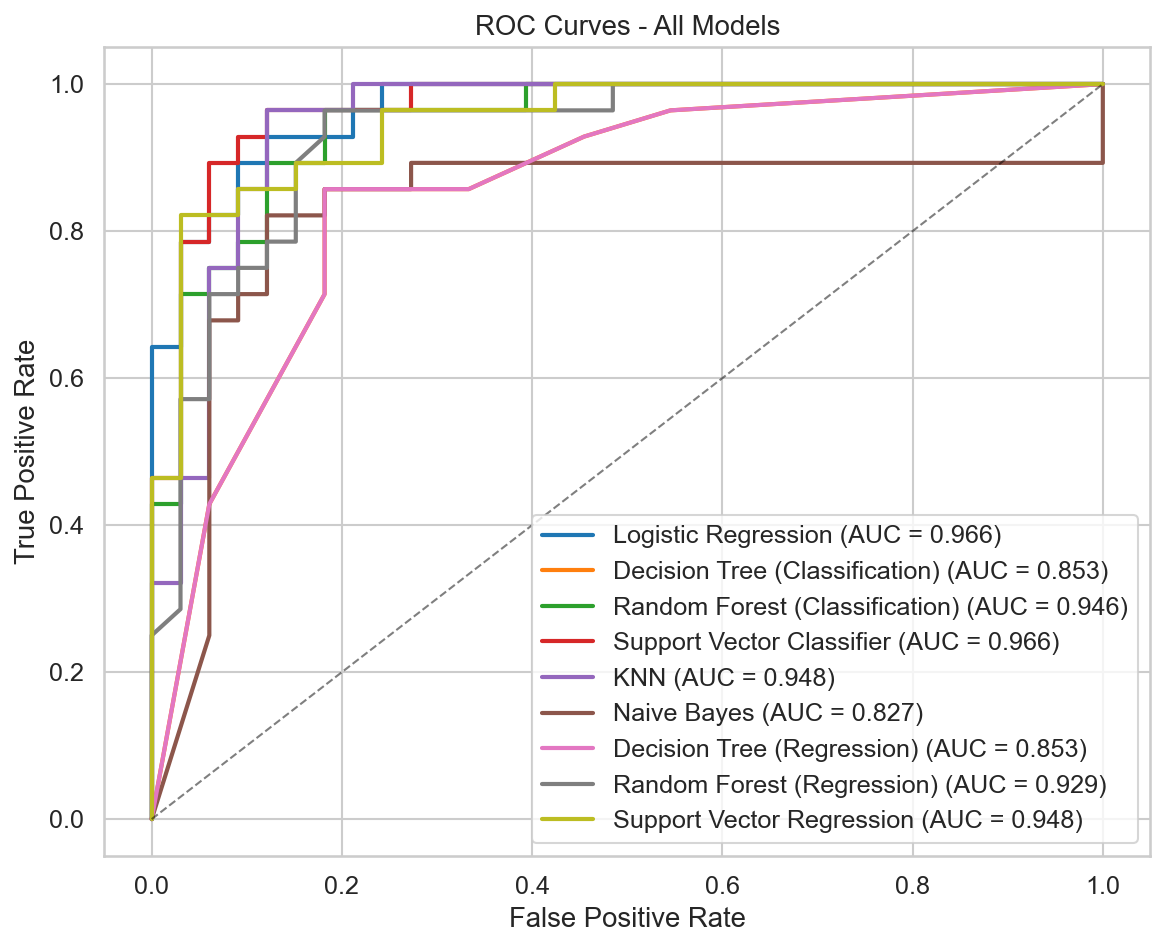
\includegraphics[width=0.95\columnwidth]{../results/figures/05_roc_curves.png}
    \caption{ROC curves for all seven tuned classifiers.}
    \label{fig:roc}
\end{figure}

\begin{figure}[h]
    \centering
    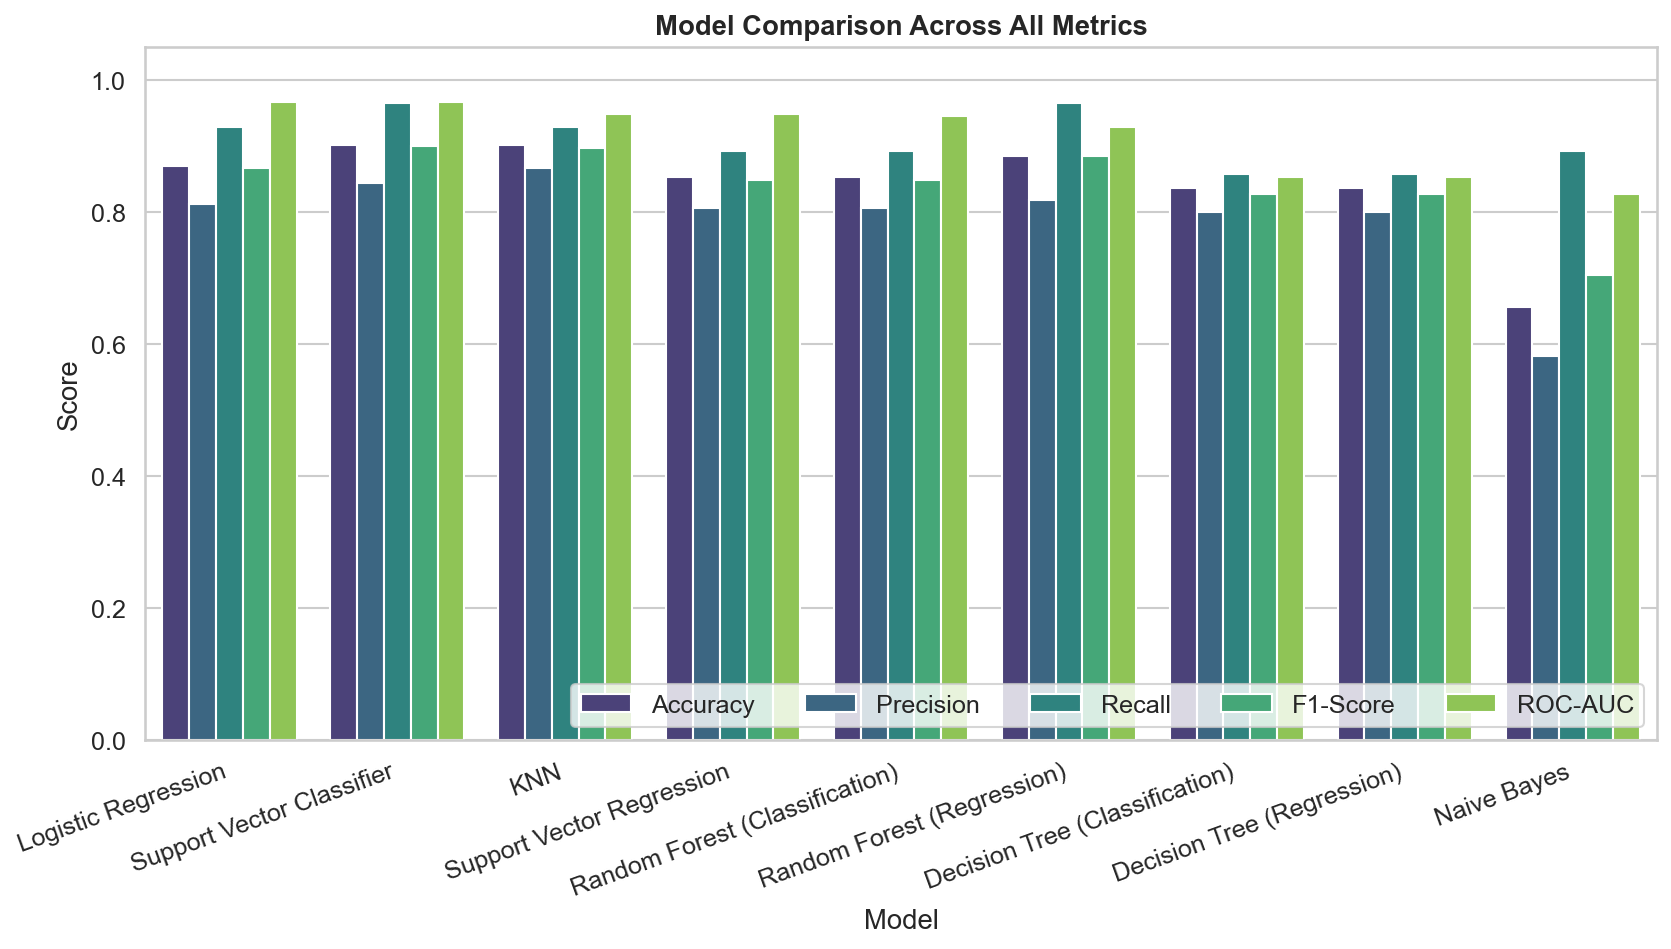
\includegraphics[width=0.95\columnwidth]{../results/figures/07_metrics_comparison.png}
    \caption{Side-by-side comparison across five evaluation metrics.}
    \label{fig:metrics}
\end{figure}

\subsection{SHAP Interpretation}
Figure~\ref{fig:shap} reports the global SHAP feature importance for the best-performing Logistic Regression model. The most influential predictors are:
\begin{enumerate}
    \item \textbf{Chest pain type (\texttt{cp})} – asymptomatic chest pain (type 4) is the single strongest signal of disease.
    \item \textbf{Number of major vessels (\texttt{ca})} – more diseased vessels correspond to higher risk.
    \item \textbf{Maximum heart rate achieved (\texttt{thalach})} – lower peak heart rate during exercise correlates with disease.
    \item \textbf{ST depression (\texttt{oldpeak})} – higher values during exercise raise risk.
    \item \textbf{Thalassemia status (\texttt{thal})} – reversible defects significantly increase predicted probability.
\end{enumerate}

These findings are clinically meaningful: every top-ranked feature is a known risk indicator in cardiology textbooks~\cite{topol2019deep}, confirming that the model has learned a medically valid representation rather than spurious correlations.

\begin{figure}[h]
    \centering
    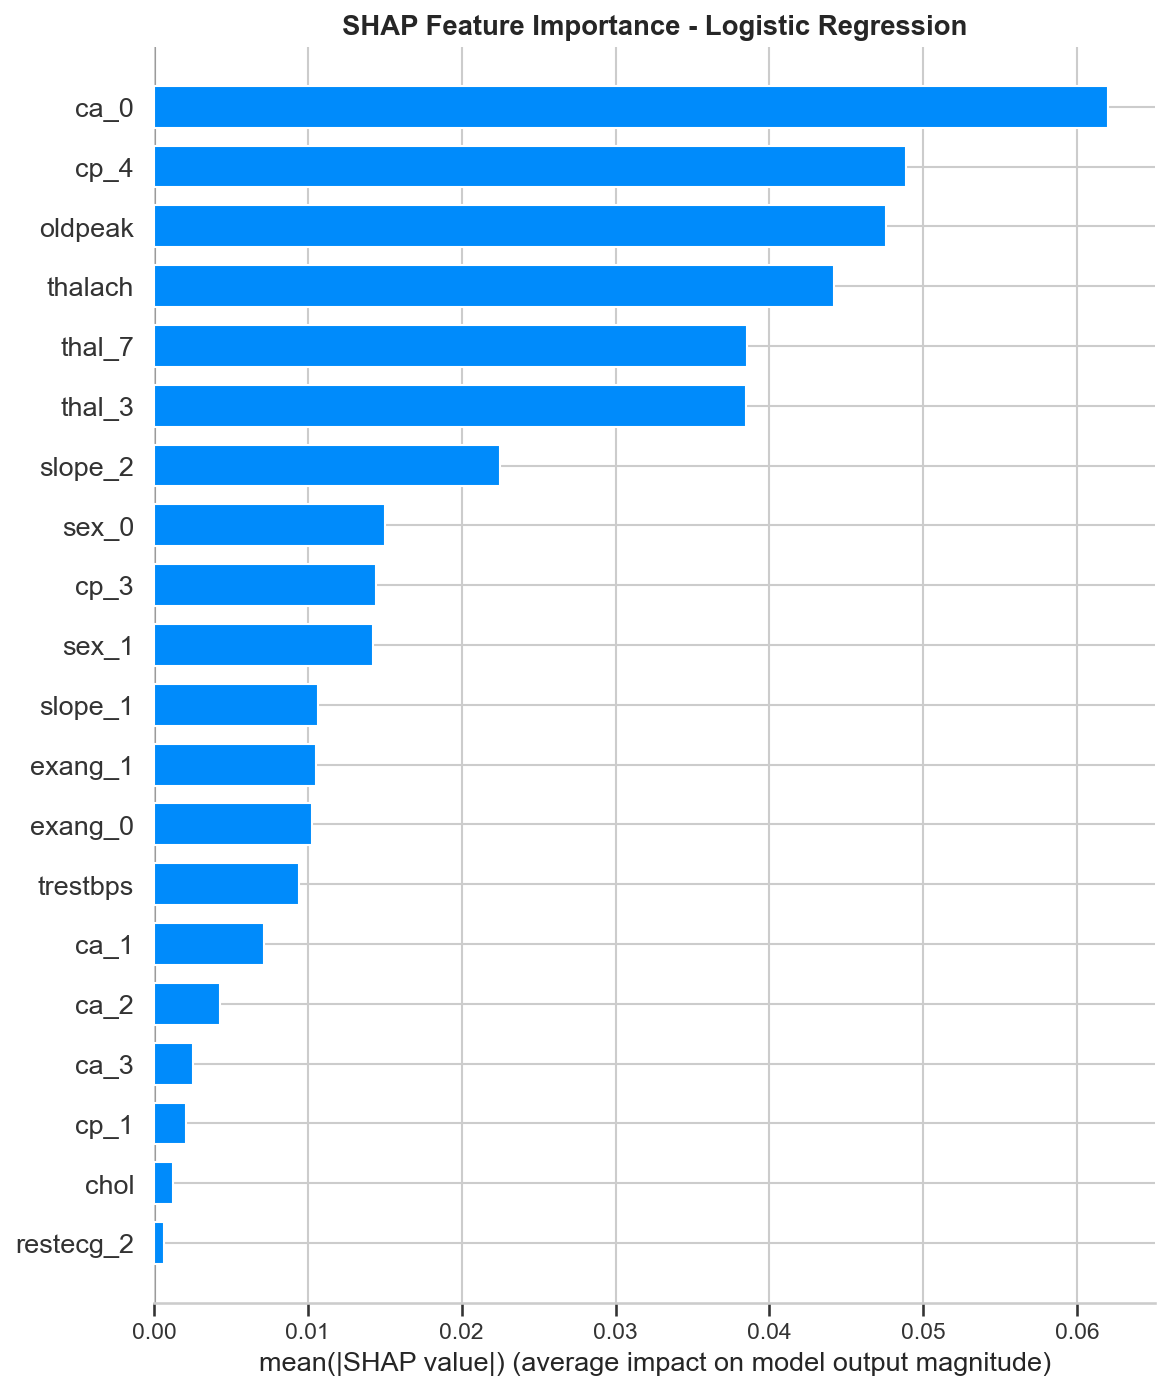
\includegraphics[width=0.95\columnwidth]{../results/figures/09_shap_bar_logistic_regression.png}
    \caption{Global feature importance via mean absolute SHAP values.}
    \label{fig:shap}
\end{figure}

\section{Web Deployment}\label{sec:deployment}
The framework is exposed as an interactive Streamlit web application (Fig.~\ref{fig:app}). A clinician enters 13 patient attributes through dropdowns and sliders; the app returns a calibrated risk probability, a categorical risk level (low / moderate / high), a verbal recommendation, and a SHAP-derived explanation of the top contributing features for that specific patient. The application also exposes the full model-comparison dashboard and the data-exploration plots, making the entire methodology reproducible and inspectable.

\begin{figure}[h]
    \centering
    \fbox{\parbox{0.93\columnwidth}{\centering Streamlit Web Demo \\[0.4em] \textit{Interactive risk gauge + SHAP waterfall explanation + four dashboards}}}
    \caption{Live demonstration interface (see \texttt{app/streamlit\_app.py}).}
    \label{fig:app}
\end{figure}

\section{Conclusion and Future Work}\label{sec:conclusion}
We have presented an end-to-end explainable AI framework for cardiovascular disease risk prediction. Among nine competing algorithms---six classifiers and three regressors adapted for binary classification---a properly tuned Logistic Regression and an RBF-kernel Support Vector Classifier jointly achieve the strongest performance (ROC-AUC = 0.966), demonstrating that simpler, interpretable models remain highly competitive on small clinical tabular datasets. The regression variants of Decision Tree, Random Forest, and SVM achieve performance broadly comparable to their classifier counterparts, validating the use of risk-score regression in CVD prediction. SHAP explanations confirm that the learned representation aligns with established cardiology knowledge, and a Streamlit web app makes the entire pipeline accessible to non-technical users.

Future work will (i) validate the framework on larger and more diverse cohorts (e.g.\ MIMIC-IV); (ii) extend it to multi-class severity prediction; (iii) incorporate temporal data through recurrent or transformer architectures; and (iv) conduct a clinical user study to evaluate the practical utility of the SHAP-based explanations in physician decision-making.

\begin{thebibliography}{00}
\bibitem{who2021cvd}
World Health Organization, ``Cardiovascular diseases (CVDs),'' WHO Fact Sheet, Geneva, 2021. [Online]. Available: \url{https://www.who.int/news-room/fact-sheets/detail/cardiovascular-diseases-(cvds)}.

\bibitem{jafar2018cardiovascular}
T. H. Jafar et al., ``Cardiovascular disease epidemic in Pakistan,'' \emph{J. Pak. Med. Assoc.}, vol. 68, no. 5, pp. 681--682, 2018.

\bibitem{krittanawong2020ml}
C. Krittanawong et al., ``Machine learning prediction in cardiovascular diseases: A meta-analysis,'' \emph{Sci. Rep.}, vol. 10, 16057, 2020.

\bibitem{ahsan2022machine}
M. M. Ahsan and Z. Siddique, ``Machine learning-based heart disease diagnosis: A systematic literature review,'' \emph{Artif. Intell. Med.}, vol. 128, 102289, 2022.

\bibitem{mienye2024deep}
I. D. Mienye and Y. Sun, ``A deep learning ensemble with data resampling for credit card fraud detection,'' \emph{IEEE Access}, vol. 10, pp. 30040--30051, 2024.

\bibitem{tjoa2021survey}
E. Tjoa and C. Guan, ``A survey on explainable artificial intelligence (XAI): Toward medical XAI,'' \emph{IEEE Trans. Neural Netw. Learn. Syst.}, vol. 32, no. 11, pp. 4793--4813, 2021.

\bibitem{lundberg2017unified}
S. M. Lundberg and S. I. Lee, ``A unified approach to interpreting model predictions,'' in \emph{Proc. NeurIPS}, 2017, pp. 4768--4777.

\bibitem{mohan2019hrflm}
S. Mohan, C. Thirumalai, and G. Srivastava, ``Effective heart disease prediction using hybrid machine learning techniques,'' \emph{IEEE Access}, vol. 7, pp. 81542--81554, 2019.

\bibitem{ali2021ensemble}
F. Ali et al., ``A smart healthcare monitoring system for heart disease prediction based on ensemble deep learning and feature fusion,'' \emph{Inf. Fusion}, vol. 63, pp. 208--222, 2020.

\bibitem{reddy2021xgboost}
G. T. Reddy et al., ``Antlion re-sampling based deep neural network model for classification of imbalanced multimodal stroke dataset,'' \emph{Multimed. Tools Appl.}, vol. 81, pp. 41801--41822, 2022.

\bibitem{detrano1989cleveland}
R. Detrano et al., ``International application of a new probability algorithm for the diagnosis of coronary artery disease,'' \emph{Am. J. Cardiol.}, vol. 64, no. 5, pp. 304--310, 1989.

\bibitem{chawla2002smote}
N. V. Chawla, K. W. Bowyer, L. O. Hall, and W. P. Kegelmeyer, ``SMOTE: Synthetic minority over-sampling technique,'' \emph{J. Artif. Intell. Res.}, vol. 16, pp. 321--357, 2002.

\bibitem{rish2001nb}
I. Rish, ``An empirical study of the Naive Bayes classifier,'' in \emph{IJCAI Workshop on Empirical Methods in AI}, 2001, pp. 41--46.

\bibitem{drucker1997svr}
H. Drucker, C. J. C. Burges, L. Kaufman, A. J. Smola, and V. Vapnik, ``Support vector regression machines,'' in \emph{Proc. NeurIPS}, 1996, pp. 155--161.

\bibitem{breiman2001rf}
L. Breiman, ``Random forests,'' \emph{Mach. Learn.}, vol. 45, no. 1, pp. 5--32, 2001.

\bibitem{rajpurkar2022aiclinical}
P. Rajpurkar et al., ``AI in health and medicine,'' \emph{Nat. Med.}, vol. 28, pp. 31--38, 2022.

\bibitem{topol2019deep}
E. J. Topol, \emph{Deep Medicine: How Artificial Intelligence Can Make Healthcare Human Again}. New York, NY: Basic Books, 2019.
\end{thebibliography}

\end{document}
